\documentclass[UKenglish]{lipics-v2016}

\usepackage{amsmath,amssymb,amsthm}
\usepackage{latexsym}
\usepackage{microtype}
\usepackage{proof}
\usepackage{stmaryrd}
\usepackage{xargs}

\usepackage{graphicx}

\usepackage{willemtools}
\usepackage{proofnet}

\bibliographystyle{plainurl}


% ============================== MACROS

\makeatletter

\theoremstyle{plain}
\newtheorem{proposition}[theorem]{Proposition}


% ===== Definitions

\newcommand\defn[1]{\textit{\textbf{#1}}}


% ===== General maths

\newcommand\floor[1]{\lfloor#1\rfloor}

% ===== Sets

\newcommand\varA{\textsc{var}^\forall}
\newcommand\varE{\textsc{var}^\exists}
\newcommand\terms{\textsc{term}}
\newcommand\termsA{\textsc{term}^\forall}
\newcommand\atom{\textsc{atom}}
\newcommand\form{\textsc{form}}
\newcommand\proofs{\textsc{proof}}
\newcommand\all{\textsc{all}}

\newcommand\ex[2]{\textsc{ex}_{#1}(#2)}

\newcommand\subs[1]{\textsc{sub}(#1)}
\newcommand\poss[1]{\textsc{pos}(#1)}
\newcommand\dom[1]{\textsc{dom}(#1)}

% ===== Formulas

\newcommand\+{+}
\renewcommand\*{\times}
\newcommand\dual[1]{\overline{#1}}

\newcommand\sub{\leq}
\newcommand\dep{\preccurlyeq}
%\newcommand\dep{\stackrel\star{\smash\preccurlyeq\rule{0pt}{1ex}}}

\newcommand\seq[3][]{{\vdash_{#1}}#2,#3}
\newcommand\fv{\textsc{fv}}

% ===== Proofs

\newcommand\prf[3]{#1\vdash\!#2,#3}

% ===== Nets

\newcommand\net[3]{#1\triangleright #2,#3}

\newcommand\deseq[4][\sigma]{[#2]_{#1}^{#3,#4}}
\newcommand\Deseq[4][\sigma]{\left[\vcenter{#2}\right]_{#1}^{#3\,,\,#4}}

%\newcommandx\deseq[4][2=\sigma]{\floor{#1}_{#2}^{#3,#4}}
%\newcommandx\Deseq[4][2=\sigma]{\left\lfloor\vcenter{#1}\right\rfloor_{#2}^{#3,#4}}

% ===== Witness maps

\newcommand\mgu{\textsc{mgu}}

\newcommand\gen{\leq}
\newcommand\coh{\smallfrown}
\newcommand\join{\vee}

\newcommand\init[2]{#1\star #2}

% ===== Slices


% ===== Coalescence

\newcommand\link[3][\sigma]{(#2,#3)_{#1}}
\newcommand\minus{\mathop{\!/\mathchoice{\kern-3pt}{\kern-3pt}{\kern-2.5pt}{\kern-2pt}/\!}}


\newcommand\scoal{\rightarrow} %{\leadsto}
\newcommand\ucoal{\rightsquigarrow}


\newcommand\qrr[1]{
  \ifx#1+\expandafter\@qrr\else
  \ifx#1*\*\mathrm R\else
  \ifx#1!\forall\mathrm R\else
  \ifx#1?\expandafter\@@qrr\else
  \ifx#11\mathrm{ax}\else
  #1\mathrm R
  \fi\fi\fi\fi\fi
}
\newcommand\@qrr[1]{+\mathrm R,#1}
\newcommand\@@qrr[1]{\exists\mathrm R,#1}
\newcommand\srr[1]{
  \ifx#1+\expandafter\@srr\else
  \ifx#1*\*\mathrm S\else
  \ifx#1!\forall\mathrm S\else
  \ifx#1?\exists\mathrm S\else 
  \ifx#11\mathrm{axS}\else
  #1\mathrm S  \fi\fi\fi\fi\fi
}
\newcommand\@srr[1]{+_{#1}\mathrm S}
\newcommand\urr[1]{
  \ifx#1+\expandafter\@urr\else
  \ifx#1*\*\mathrm U\else
  \ifx#1!\forall\mathrm U\else
  \ifx#1?\exists\mathrm U\else 
  \ifx#11\mathrm{axU}\else
  #1\mathrm U
  \fi\fi\fi\fi\fi
}
\newcommand\@urr[1]{+_{#1}\mathrm U}

% ===== Derivations

\newcommand\sdown{\mathrel{\rotatebox[origin=c]{-90}{$\scoal$}\kern1pt}}
\newcommand\udown{\mathrel{\rotatebox[origin=c]{-90}{$\ucoal$}\kern1pt}}

\newcommandx\sdn[4][2=\sigma]{#1\sdown\link[#2]{#3}{#4}}	%{#2\sdown_{#1}{#3}\mathbin,{#4}}
\newcommandx\udn[4][2=\sigma]{#1\udown\link[#2]{#3}{#4}}	%{#2\udown_{#1}{#3}\mathbin,{#4}}

% ===== (De-)Sequentialization

\newcommand\QU{\Leftrightarrow}


\makeatother

% ============================== TITLE & AUTHORS

\title{Proof nets for first-order additive linear logic}
%\titlerunning{Proof nets for ALL1}


\author[1]{Willem B.\ Heijltjes}
\author[2]{Dominic J.D.\ Hughes}
\author[3]{Lutz Stra\ss burger}
\affil[1]{University of Bath, United Kingdom\\
  \texttt{w.b.heijltjes@bath.ac.uk}}
\affil[2]{
  \texttt{}}
\affil[3]{INRIA \&\ \'Ecole Polytechnique, Palaiseau, France\\
  \texttt{lutz.strassburger@inria.fr}}
\authorrunning{W.B.\ Heijltjes, D.J.D.\ Hughes, and L.\ Stra\ss burger}

\Copyright{Willem B.\ Heijltjes, Dominic J.D.\ Hughes, and Lutz Stra\ss burger}

\subjclass{Dummy classification -- please refer to \url{http://www.acm.org/about/class/ccs98-html}}% mandatory: Please choose ACM 1998 classifications from http://www.acm.org/about/class/ccs98-html . E.g., cite as "F.1.1 Models of Computation". 
\keywords{Linear logic, Proof nets}


% ============================== CONTENT

\begin{document}

\maketitle

\begin{abstract}

\end{abstract}

\subsection{Proof identity}

\[
	\infer={\exists x.p(x),\exists y.\dual p(y)}{\infer{p(t),\dual p(t)}{}}
	\quad
	\stackrel?\equiv
	\quad
	\infer={\exists x.P(x),\exists y.\dual p(y)}{\infer{p(s),\dual p(s)}{}}
\]

\[
	\infer{\exists x.p,\dual p}{\infer{p[t/x],\dual p}{}}
	\quad
	\stackrel?\equiv
	\quad	
	\infer{\exists x.p,\dual p}{\infer{p[s/x],\dual p}{}}
\]

\[
	\infer{\exists x.p\+q(x),\dual p}{\infer{p\+q(t)}{\infer{p,\dual p}{}}}
	\quad
	\stackrel?\equiv
	\quad	
	\infer{\exists x.p\+q(x),\dual p}{\infer{p\+q(s)}{\infer{p,\dual p}{}}}
\]

\[
\begin{tikzpicture}[net]
\formula[y=1]{\exists x.\forall a.~p(a,x)}
\formula[y=0]{\exists y.~{\dual p}(y,s)\*{\dual p}(y,t)}
\Vlink[red,label={$\scriptstyle\sigma~$},l]{[-2]8,5}
\Vlink[red,label={$~\scriptstyle\tau$}]{[2]8,12}
\end{tikzpicture}
\]

\[
\begin{tikzpicture}[net]
\formula[y=1]{\exists x.\forall a.~p(a,x)}
\formula[y=0]{\exists y.~{\dual p}(y,s)\*{\dual p}(y,t)}
\Vlink[red,label={$~\scriptstyle\upsilon$}]{8,11}
\end{tikzpicture}
\]

\[
\begin{tikzpicture}[net]
\formula[y=1]{\exists x.\forall a.~p(a,x)}
\formula[y=0]{\exists y.~{\dual p}(y,s)\*{\dual p}(y,t)}
\Vlink[red,label={$\quad\scriptstyle{\upsilon\minus y}$}]{8,1}
\end{tikzpicture}
\]

\[
\begin{tikzpicture}[net]
\formula[y=1]{\exists x.\forall a.~p(a,x)}
\formula[y=0]{\exists y.~{\dual p}(y,s)\*{\dual p}(y,t)}
\Vlink[red,label={$~\scriptstyle{\upsilon\minus y}$}]{4,1}
\end{tikzpicture}
\]

\[
\begin{tikzpicture}[net]
\formula[y=1]{\exists x.\forall a.~p(a,x)}
\formula[y=0]{\exists y.~{\dual p}(y,s)\*{\dual p}(y,t)}
\Vlink[red,label={$~\scriptstyle{\rho}$}]{1,1}
\end{tikzpicture}
\]

\[
	\sigma = [a/y, s/x]
	\qquad
	\tau = [a/y, t/x]
\]
\[
	\upsilon = \rho[a/y, u/x]
	\qquad
	\rho = \mgu(s,t)
	\qquad
	 u=s\rho=t\rho
\]


% ==================================================

\section{Proof nets for first-order additive linear logic}

% ..................................................

%\begin{figure}
%\[
%	\infer{\seq P{\dual P}}{}
%\qquad
%	\infer{\seq A{B_0\+B_1}}{\seq A{B_i}}
%\qquad
%	\infer{\seq A{B\*C}}{\seq AB && \seq AC}
%\qquad
%	\infer{\seq A{\exists x.B}}{\seq A{B[t/x]}}
%\qquad
%	\infer[\!\!\scriptstyle{a\,\notin\,\textsc{fv}(A)}]{\seq A{\forall a.B}}{\seq AB}
%\]
%\caption{A sequent calculus for $\all1$}
%\label{fig:sequent calculus}
%\end{figure}

\begin{figure}
\[
	\infer[\!\!\scriptstyle{\qrr1}]{\seq P{\dual P}}{}
\quad
	\infer[\!\!\scriptstyle{\qrr+i}]{\seq A{B_0\+B_1}}{\seq A{B_i}}
\quad
	\infer[\!\!\scriptstyle{\qrr*}]{\seq A{B\*C}}{\seq AB & \seq AC}
\quad
	\infer[\!\!\scriptstyle{\qrr?t}]{\seq A{\exists x.B}}{\seq A{B[t/x]}}
\quad
	\infer[\!\!\scriptstyle{\qrr!~(a\,\notin\,\textsc{fv}(A))}]{\seq A{\forall a.B}}{\seq AB}
\]
\caption{A sequent calculus for $\all1$}
\label{fig:sequent calculus}
\end{figure}
%
%\begin{figure}
%\[
%\raisebox{.5ex}{$\qrr1$}\quad
%	\infer{\seq P{\dual P}}{}
%\quad\raisebox{.5ex}{$\qrr+i$}\quad
%	\infer{\seq A{B_0\+B_1}}{\seq A{B_i}}
%\quad\raisebox{.5ex}{$\qrr*$}\quad
%	\infer{\seq A{B\*C}}{\seq AB && \seq AC}
%\quad\raisebox{.5ex}{$\qrr?$}\quad
%	\infer{\seq A{\exists x.B}}{\seq A{B[t/x]}}
%\quad\raisebox{.5ex}{$\qrr!$}\quad
%	\infer[\!\!\scriptstyle{a\,\notin\,\textsc{fv}(A)}]{\seq A{\forall a.B}}{\seq AB}
%\]
%\caption{A sequent calculus for $\all1$}
%\label{fig:sequent calculus}
%\end{figure}



% ..................................................

% --------------------------------------------------

\subsection{First-order additive linear logic}

First-order terms and the formulas of first-order $\all$ are generated by the following grammars.
%
\setMidspace{5pt}
\[
\begin{array}{@{}l@{}l}
	t &\Coloneqq a \Mid x \Mid f(t_1,\dots,t_n)
\\[10pt]
	P &\Coloneqq p(t_1,\dots,t_n) \Mid \dual p(t_1,\dots,t_n)
\\[10pt]
	A &\Coloneqq P \Mid A\+A \Mid A\*A \Mid \exists x.A \Mid \forall a.A
\end{array}
\]
%
Negation $(\dual{\,\cdot\,})$ is applied to predicate symbols, $\dual p$, as a matter of convenience. The \defn{dual} $\dual A$ of an arbitrary formula $A$ is given by DeMorgan. We use the following notational conventions.
%
\[
\begin{tabular}{@{}lll@{}}
	$a,b,c$ & $\in \varA$ 		& universally quantified variables (and free variables)\\
	$x,y,z$ & $\in \varE$		& existentially quantified variables (and term-language variables)\\
	$f,g,h$ & $\in \Sigma_f$	& $n$-ary $(n\geq 0)$ function symbols from a fixed alphabet $\Sigma_f$\\
	$p,q,r$ & $\in \Sigma_p$	& $n$-ary $(n\geq 0)$ predicate symbols from a fixed alphabet $\Sigma_p$ \\
	$s,t,u$ & $\in \terms$ 		& first-order terms over $\varA$, $\varE$, $\Sigma_f$, and $\Sigma_p$ \\
	$P,Q,R$ & $\in \atom$		& atomic propositions \\
	$A,B,C$ & $\in \form$		& \all1 formulas \\
\end{tabular}
\]
%
A \defn{sequent} $\seq AB$ is a pair of formulas $A$ and $B$. A sequent calculus for \all1 is given in Figure~\ref{fig:sequent calculus}, where each rule has a symmetric counterpart that applies to the first formula in the sequent. We write $\prf\pi AB$ for a proof $\pi$ with conclusion sequent $\seq AB$.

By a \defn{subformula} we will mean a subformula \defn{occurrence}. For instance, a formula $A\*A$ has two subformulas $A$, one on the left and one on the right. The \defn{subformulas} $\subs A$ of a formula are defined as follows; we write $B\sub A$ if $B$ is a subformula of $A$, i.e.\ if $B\in\subs A$.
\[
	\subs A = \{A\} \cup
	\left\{\begin{array}{ll}
		\subs B\uplus\subs C	& \text{if $A=B\+C$ or $A=B\*C$} \\[5pt]
		\subs B					& \text{if $A=\exists x.B$ or $A=\forall a.B$}
	\end{array}\right.
\]

A \defn{link} $(C,D)$ on a sequent $\seq AB$ is a pair of subformulas $C\leq A$ and $D\leq B$. 
A \defn{linking} $\lambda$ on the sequent $\seq AB$ is a set of links on it.

\begin{definition}
A \defn{pre-net} $\net\lambda AB$ is a sequent $\seq AB$ with a linking $\lambda$ on it.
\end{definition}


% --------------------------------------------------

\subsection{Witness maps}

A \defn{witness map} $\sigma\colon \varE \rightharpoonup \terms$ is a substitution map which assigns terms to existential variables, given as a (finite) partial function. Its \defn{domain} $\dom(\sigma)$ are those variables for which it is defined. The \defn{empty} witness map $\varnothing$ is the everywhere undefined partial function, and the map $\sigma[t/x]$ substitutes $t$ for $x$ and is as $\sigma$ everywhere else. We express by $\sigma(x)=\bot$ that $\sigma$ is undefined for $x$. The map $\sigma\minus x$ is undefined on $x$ and otherwise as $\sigma$. 

We will write $A\sigma$ for the application of the witness map $\sigma\colon\varE\rightharpoonup\terms$ to the formula $A$ as a substitution map. It is applied to a sequent proof, $\pi\sigma$, by applying it to each formula in the proof $\pi$. The \defn{composition} of two maps is written $\sigma\tau$, where $A(\sigma\tau)=(A\sigma)\tau$.

A \defn{witness linking} $\lambda_\Sigma$ is a linking $\lambda$ with a \defn{witness labelling} $\Sigma\colon\lambda\to \varE\rightharpoonup\terms$ that assigns each link $(C,D)$ a witness map. We may use and define $\lambda_\Sigma$ as a set of \defn{witness links} $\link CD$, where $(C,D)$ in $\lambda$ and $\Sigma(C,D)=\sigma$. When link is not a witness link may be emphasized by calling it \defn{clean}.

\begin{definition}
A \defn{witness pre-net} $\net{\lambda_\Sigma}AB$ is a sequent $\seq AB$ with a witness linking $\lambda_\Sigma$.
%
%\begin{description}
%	\item[Exact coverage]
%The domain of $\sigma$ is exactly the variables existentially quantified in $\seq AB$ that will be bound in $C$ and $D$, if they occur:
%\[
%	\dom\sigma = \{\,x \mid C < \exists x.X \leq A\,\}
%			\cup \{\,y \mid D < \exists y.Y \leq B\,\}~.
%\]
%
%	\item[Eigenvariables not free]
%A universal variable $a\in\varA$ quantified in $C$ or $D$ may not occur free in the range of $\sigma$, $a\notin\sigma$.
%
%	\item[Freshness]
%Existential variables in the range of $\sigma$ are fresh, i.e.\ distinct from any existentially quantified variable in $\seq AB$.
%\end{description}
\end{definition}

We will assume the following variable naming conventions for \all1 pre-nets.

\begin{description}
	\item
[\defn{Barendregt's convention}] All quantifiers in a sequent $\seq AB$ have a distinct binding variable, and no bound variable shares a name with a free one.
%	\item
%% ALTERNATIVE: "STATIC WITNESSING"
%[\defn{Universal witnessing}] All existential witnesses in a proof are \defn{universal terms} $\termsA\subset\terms$, generated by the following grammar.
%\[
%	\termsA: \qquad t \Coloneqq a \Mid f(t_1,\dots,t_n)
%\]

	\item[Eigenvariables not free]
For a link $\link CD$, a universal variable $a\in\varA$ quantified in $C$ or $D$ may not occur free in the range of $\sigma$, $a\notin\sigma$.

	\item[Freshness]
For a link $\link CD$, existential variables in the range of $\sigma$ are fresh, i.e.\ distinct from any existentially quantified variable in $\seq AB$.
\end{description}


%We assume the existential variables occurring in the range of $\Sigma$ to be fresh, i.e.\ distinct from any existentially quantified variable in $\seq AB$.  
We abbreviate by $a\in \sigma$ the statement that a variable $a$ occurs free in the range of $\sigma$, i.e.\ that $a\in\fv(\sigma(x))$ for some $x$.

\begin{definition}
The \defn{de-sequentialization} $[\pi]$ of a sequent proof $\prf\pi AB$ is the witness pre-net $\net{\lambda_\Sigma}AB$ where $\lambda_\Sigma=\deseq[\varnothing]\pi AB$ and $\deseq-AB$ is defined as follows.
%
\newlength\deseqwidth
\settowidth\deseqwidth{$\scriptstyle{A'\,,\,B'_0\+B'_1}$}
\newcommand\XDeseq[4][\sigma]{\left[\vcenter{#2}\right]_{#1}^{\makebox[\deseqwidth][l]{$\scriptstyle{#3\,,\,#4}$}}}
\begin{align*}
	\XDeseq{\infer{\seq P{\dual P}}{}}QR &\quad=\quad \{\link QR\}
\\ \\
	\XDeseq{\infer {\seq A {B_0\+B_1}} {\deduce [\rule{0pt}{1pt}] {\seq A{B_i}} \pi }}
	  {A'}{B_0'\+B'_1} 
	& \quad=\quad 
	\Deseq{\deduce[\rule{0pt}{1pt}]{\seq A{B_i}}\pi}{A'}{B_i'}
\\ \\
	\XDeseq{\infer{\seq A{B\*C}}{
	  \deduce[\rule{0pt}{1pt}]{\seq AB}\pi 
	  && 
	  \deduce[\rule{0pt}{1pt}]{\seq AC}\Sigma}}{A'}{B'\*C'}
	& \quad=\quad 
	  \Deseq{\deduce[\rule{0pt}{1pt}]{\seq AB}\pi}{A'}{B'}
	  \cup
	  \Deseq{\deduce[\rule{0pt}{1pt}]{\seq AC}\Sigma}{A'}{C'}
\\ \\
	\XDeseq{\infer{\seq A{\exists x.B}}{\deduce[\rule{0pt}{1pt}]{\seq A{B[t/x]}}\pi}}
	  {A'}{\exists x.B'}
	& \quad=\quad 
	 \Deseq[{\sigma[t/x]}]{\deduce[\rule{0pt}{1pt}]{\seq A{B[t/x]}}\pi}
	  {A'}{B'}
\\ \\
	\XDeseq{\infer[\!\!\scriptstyle{a\,\notin\,\textsc{fv}(A)}]
	  {\seq A{\forall a.B}}{\deduce[\rule{0pt}{1pt}]{\seq AB}\pi}}{A'}{\forall a.B'}
	& \quad=\quad 
	  \Deseq{\deduce[\rule{0pt}{1pt}]{\seq AB}\pi}{A'}{B'}
\end{align*}
\end{definition}


A witness link $\link PQ$ on two atomic formulas $P$ and $Q$ is an \defn{axiom} link if $P\sigma=\dual Q\sigma$; a witness \defn{axiom} linking is one where every link is an axiom link. Observe that the de-sequentialization $[\pi]$ is a witness pre-net with axiom linking $\deseq[\varnothing]\pi AB$.


% --------------------------------------------------

\subsection{Correctness and sequentialization}

Correctness and sequentialization for \all1 proof nets will be through \defn{coalescence}. This is a simple graph rewriting relation that gives top-down sequentialization, from the axioms to the conclusion of a proof. It is the additive counterpart to Danos \defn{contractibility} for multiplicative linear logic. 

We will define two coalescence relations, one \defn{strict} $(\scoal)$, for witness nets, and one \defn{unifying} $(\ucoal)$, for unification nets, in a later section. In the former, to join two slices the witness assignment must be the same; in the latter, witness assignments must be compatible, so that a common, more general witness map exists. 

For sequentialization, the links in a pre-net will be labelled with a sequent proof. An axiom link will carry an axiom, and each coalescence step introduces one proof rule. Formalizing this, a \defn{proof linking} $\lambda_\Sigma^\Pi$ is a witness linking $\lambda_\Sigma$ with a \defn{proof labelling} $\Pi\colon \lambda\to\proofs$ assigning each link a sequent proof. We will use and define $\lambda_\Sigma^\Pi$ as a set of \defn{proof links} $\link CD^\pi$, where we require that $\prf\pi{C\sigma}{D\sigma}$, i.e.\ that $\pi$ proves the conclusion $\seq{C\sigma}{D\sigma}$. A \defn{labelled pre-net} $\net{\lambda_\Sigma^\Pi}AB$ is a witness pre-net $\net{\lambda_\Sigma}AB$ with a proof labelling $\Pi$ on $\lambda_\Sigma$. The \defn{initial proof labelling} $\lambda_\Sigma^\star$ of an axiom linking $\lambda_\Sigma$ is:
\[
	\lambda_\Sigma^\star = \{~\link PQ^\pi~\mid~\link PQ\in\lambda_\Sigma~,~\pi=~\infer{\seq{P\sigma}{Q\sigma}}{}~\}~.
\]
For correctness we may coalesce a pre-net directly, without constructing a proof. 

To recap, we have accumulated the following further notational conventions.
%
\[
\begin{tabular}{@{}lcll@{}}
	$\kappa,\lambda$ 	& $\subset$ & $\form\times\form$ 	& linkings (sets of pairs of formulas)\\
	$\rho,\sigma,\tau$	& $\colon$  & $\varE\rightharpoonup\terms$ & witness maps\\
	$\Sigma,\Xi$		& $\colon$  & $(\form\times\form)\rightharpoonup\varE\rightharpoonup\terms$		& witness labellings on a linking \\
	$\pi,\phi,\psi$		& $\in$ & $\proofs$ & \all1 sequent proofs\\
	$\Pi,\Phi,\Psi$		& $\colon$  & $(\form\times\form)\rightharpoonup\proofs$		& proof labellings on a linking
\end{tabular}
\]

\begin{definition}
 \defn{Strict sequentialization} ($\scoal$) is the rewrite relation on witness pre-nets generated by the following rules, which apply symmetrically to the first formula in the sequent. \defn{Strict coalescence} is the same relation ignoring proof labels, on witness pre-nets.
%
\renewcommand{\+}{{+}}
\renewcommand{\*}{{\times}}
\begin{equation}
  	\net{\{\link A{B_i}^\pi\}}A{B_0\+B_1} 
 ~\scoal~
	\net{\{\link A{B_0\+B_1} ^\psi\}}A{B_0\+B_1}
\tag{$\srr+i$}
\end{equation}

\hfill $\text{where}\quad \psi=~
  \vc{
   \infer  {\seq{A\sigma}{B_0\sigma\,\+\,B_1\sigma}}  {
  	\deduce  [\rule{0pt}{1pt}]  {\seq{A\sigma}{B_i\sigma}}  \pi
  }}
$ \hspace*{20pt}

\begin{equation}
	\net{\{\link AB^\pi,\link AC^\phi\}}A{B\*C}
 ~\scoal~ 
	\net{\{\link A{B\*C}^\psi\}}A{B\*C}
\tag{$\srr*$}
\end{equation}

\hfill $\text{where}\quad \psi=~
  \vc{
   \infer  {\seq{A\sigma}{B\sigma\,\*\,C\sigma}}  {
    \deduce  [\rule{0pt}{1pt}]  {\seq{A\sigma}{B\sigma}}  \pi
    &
    \deduce  [\rule{0pt}{1pt}]  {\seq{A\sigma}{C\sigma}}  \phi    
  }}$ \hspace*{20pt}

\begin{equation}
	\net{\{\link AB^\pi\}}A{\exists x.B}
 ~\scoal~ 
	\net{\{\link[\sigma\minus x]A{\exists x.B}^\psi\}}A{\exists x.B}
\tag{$\srr?$}
\end{equation}

\hfill $\text{if}\quad\sigma(x)\,\neq\,\bot~,
		\quad
		\text{where}\quad \tau=\sigma\minus x
		\quad
		\text{and}\quad \psi=~
  \vc{
   \infer  {\seq{A\tau}{\exists x.B\tau}}  {
    \deduce  [\rule{0pt}{1pt}]  {\seq{A\sigma}{B\sigma}}  \pi  
  }}
$ \hspace*{20pt}

\begin{equation}
	\net{\{\link AB\}}A{\forall a.B}
 ~\scoal~
	\net{\link A{\forall a.B}}A{\forall a.B}
\tag{$\srr!$}
\end{equation}

\hfill $\text{if}\quad a\notin\sigma~,
		\quad
		\text{where}\quad \psi=~
  \vc{
   \infer  {\seq{A\sigma}{\forall a.B\sigma}}  {
    \deduce  [\rule{0pt}{1pt}]  {\seq{A\sigma}{B\sigma}}  \pi  
  }}
$ \hspace*{20pt}

\medskip

\noindent
A witness pre-net $\net{\lambda_\Sigma}AB$ \defn{strict-coalesces} if it reduces to a single link $\net{\{\link[\varnothing]AB\}}AB$.\end{definition}


To be explicit, to generate coalescence as a rewrite relation means the following: a pre-net coalesces to another, $\net{\lambda_\Sigma} AB\scoal \net{{\lambda'_{\Sigma'}}}AB$ if and only if there is a rewrite rule
\[
	\net{\kappa_\Xi} CD\scoal\net{\kappa'_{\Xi'}} CD
\] 
such that 
\[
	C\leq A \qquad
	D\leq B \qquad
	\kappa_\Xi\subseteq\lambda_\Sigma \qquad
	\kappa'_{\Xi'}\subseteq\lambda'_{\Sigma'} \quad
	\text{and} \quad
	\lambda_\Sigma-\kappa_\Xi=\lambda'_{\Sigma'}-\kappa'_{\Xi'}~.
\]

\begin{definition}
An \all1 \defn{witnessing proof net} or \defn{witness net} is a witness pre-net $\net{\lambda_\Sigma}AB$, with $\lambda_\Sigma$ an axiom linking, that strict-coalesces. It \defn{sequentializes} to a proof $\pi$ if its initial labelling $\net{\lambda_\Sigma^\star}AB$ reduces in $(\scoal)$ to $\net{\{\link[\varnothing]AB^\pi\}}AB$.
\end{definition}

Two useful properties of witness nets are preserved over a coalescence sequence, captured in the lemma below. The first property is formulated the way it is to account for vacuous quantifiers, for which no actual variable occurs in $C$ or $D$, as well as formulas such as $\exists x.C\+C'$ where $x$ occurs in $C'$ but not $C$, where we still would like an explicit witness for $x$ on a link $\link CD$. 


\begin{lemma}
Every pre-net on a coalescence path $\net{\lambda_\Sigma}AB \scoal^* \net{\{\link[\varnothing]AB^\pi\}}AB$ from a witness net satisfies the \defn{exact coverage} property: for any link $\link CD$, the domain of $\sigma$ is exactly the variables existentially quantified in $\seq AB$ thad bind in $C$ and $D$,
\[
	\dom\sigma = \{\,x \mid C < \exists x.X \leq A\,\}
			\cup \{\,y \mid D < \exists y.Y \leq B\,\}~.
\]
\end{lemma}

%
%\begin{lemma}
%Every pre-net on a coalescence path $\net{\lambda_\Sigma}AB \scoal^* \net{\{\link[\varnothing]AB^\pi\}}AB$ from a witness net satisfies the following properties. 
%\begin{description}
%	\item[Eigenvariables not free]
%For any link $\link CD$, a universal variable $a\in\varA$ quantified in $C$ or $D$ does not occur free in the range of $\sigma$, $a\notin\sigma$.
%
%	\item[Exact coverage]
%For any link $\link CD$, the domain of $\sigma$ is exactly the variables existentially quantified in $\seq AB$ that will be bound in $C$ and $D$, if they occur:
%\[
%	\dom\sigma = \{\,x \mid C < \exists x.X \leq A\,\}
%			\cup \{\,y \mid D < \exists y.Y \leq B\,\}~.
%\]
%\end{description}
%\end{lemma}

\begin{proof}
By induction on the coalescence path, going forward from $\net{\lambda_\Sigma}AB$ for the first property, and working backward from $\net{\{\link[\varnothing]AB^\pi\}}AB$ for the second.
\end{proof}


\begin{theorem}
For any \all1 proof $\pi$, the de-sequentialization $[\pi]$ is a witness net that sequentializes to $\pi$. 
\end{theorem}

\begin{proof}
It follows by induction on $\prf\pi AB$ that if $\lambda_\Sigma=[\pi]_{A',B'}^\sigma$ where $A'\sigma=A$ and $B'\sigma=B$, then $\net{\lambda^\star_\Sigma}AB$ reduces in $(\scoal)$ to $\net{\{\link{A'}{B'}^\pi\}}AB$. The statement is the specific case $\sigma=\varnothing$.
\end{proof}


% --------------------------------------------------

\subsection{Geometric correctness}

%A formula $\exists x.A$ has two natural immediate descendants: one \emph{syntactic}, its subformula $A$, and one \emph{semantic}, the premise $A[t/x]$ for its introduction rule, for any given $t$. We will define the latter as a tree-order generated from a formula $A$: the \defn{positions} of $A$ are its subformulas under substitution,
%\[
%	\poss A~=~\{~B'\sigma~\mid~A=A'\sigma~,~B'\sub A'~,~\sigma\in\varE\rightharpoonup\terms~\}
%\]

A \defn{slice} is the fraction of a proof that depends on a given choice of one branch (or projection) on each product formula $A\*B$. Important to additive proof theory is that many operations can be performed on a per-slice basis, such as normalization, or proof net correctness. We will here use slices for the latter purpose.

As in the propositional case, we define a slice of a sequent $\seq AB$ as a set of potential links, of which exactly one must be realized in a proof net $\net{\lambda_\Sigma}AB$.

%In the propositional case, slices are readily defined as sets of subformulas. Here, in the first-order case, we will need to 

%The immediate problem is that the number of positions immediately below $\exists x.B$ is infinite, as there is one immediate descendant $B[t/x]$ for every term $t$. We reduce it to finite width by restricting a slice to just the terms assigned to $x$ by the witness labelling $\Sigma$ in a pre-net $\net{\lambda_\Sigma}AB$.

For a witness linking $\lambda_\Sigma$ and an existential variable $x$, write $\Sigma(x)\subseteq\terms$ for the \defn{witness set} of $x$, which collects the terms assigned to $x$ by the witness maps in $\Sigma$ for every link in $\lambda$:
\[
	\Sigma(x) = \{~\sigma(x)~\mid~\link CD\in\lambda_\Sigma~\}~.
\]
%
Given a witness linking $\lambda_\Sigma$, a \defn{slice} $S$ of a formula $A$ and a witness map $\sigma$ is a set of pairs $(A',\sigma)$ where $A'$ is a subformula of $A$, given by: $S=\{(A,\sigma)\}\cup S'$ where $S'$ is as follows.
%
\begin{itemize}
	\item
\makebox[70pt][l]{If $A = P$}			then $S'=\varnothing$.
	\item
\makebox[70pt][l]{If $A = B\+C$} 		then $S'=S_B\uplus S_C$ where $S_B$ is a slice of $B$ and $\sigma$, and $S_C$ a slice of $C$ and $\sigma$.
	\item
\makebox[70pt][l]{If $A = B\*C$}		then $S'$ is a slice of $B$ and $\sigma$ or a slice of $C$ and $\sigma$.
	\item
\makebox[70pt][l]{If $A = \exists x.B$}	then $S'=\uplus_{t\,\in\,\Sigma(x)}S_t$ where each $S_t$ is a slice of $B$ and $\sigma[t/x]$.
	\item
\makebox[70pt][l]{If $A = \forall a.B$}	then $S'$ is a slice of $B$ and $\sigma$.
\end{itemize}
%
\noindent
A \defn{slice} of a sequent $\seq AB$ is a set of links
\[
	\{~\link[\sigma\cup\tau]CD~\mid~(C,\sigma)\in S_A~,~(D,\tau)\in S_B~\}
\]
where $S_A$ is a slice of $A$ and $\varnothing$, and $S_B$ a slice of $B$ and $\varnothing$.  A \defn{slice} of a witness pre-net $\net{\lambda_\Sigma} AB$ is the intersection $\lambda_\Sigma\cap S$ of $\lambda_\Sigma$ with a slice $S$ of $\seq AB$.

Within a slice, we need to ensure that the order in which quantifiers are instantiated is sound. That is, we need to have an analogue of the \emph{eigenvariable condition} on the $\qrr!$-rule of sequent calculus, that the quantified variable $a$ of the primary formula $\forall a.A$ does not occur free in the context. We will define a \defn{dependency} condition to this effect.

Since we will require that each slice contains a single link, for simplicity we will define the dependency condition on individual links rather than on slices. It is expected that for a more involved logic that includes multiplicative connectives, a dependency condition such as the below one needs to be applied to a slice instead.

For a subformula $C$ of a formula $A$, let the \defn{existential covering} $\ex AC$ of $C$ be the set of variables that are existentially quantified in $A$ dominating $C$:
\[
	\ex AC = \{\,x \mid C < \exists x.X \sub A\,\}
\]
In a pre-net $\net{\lambda_\Sigma}AB$, let the \defn{column} of a link $\link CD$ be the set of pairs 
\[
	\{~(X,\sigma|\ex AX)~\mid~C\sub X\sub A~\}\cup\{~(Y,\sigma|\ex BY)~\mid~D\sub Y\sub B~\}~,
\]
with an order $(\dep)$ given by: $(X,\rho)\dep(Y,\tau)$ if $X\leq Y$, or $Y$ occurs as $\forall a.Y$ and $a\in\rho$.

\begin{definition}
A witness pre-net is \defn{correct} if it is
\begin{enumerate}
\item \defn{slice-correct}: every slice is a singleton, and
\item \defn{dependency-correct}: every column is a partial order (i.e.\ is acyclic/antisymmetric).
\end{enumerate}
\end{definition}


\begin{lemma}
\label{lem:preservation}
Strict coalescence preserves and reflects correctness: for a strict coalescence step $L\scoal R$, the witness pre-net $L$ is correct if and only if $R$ is.
\end{lemma}

\begin{proof}
Let $L=\net{\lambda_\Sigma}AB$ and $R=\net{\kappa_\Xi}AB$. We will consider the four coalescence steps as shown below. For slice-correctness, we will demonstrate that the left-hand side and right-hand side of each rule belong to the same slice of $\seq AB$, or in the case of $\srr?$, naturally corresponding slices.
%
\begin{align}
  	\net{\{\link C{D_i}\}}C{D_0{\+}D_1} 
 &~\scoal~
	\net{\{\link C{D_0{\+}D_1} \}}C{D_0{\+}D_1}
\tag{$\srr+i$}
\\	\net{\{\link C{D_0},\link C{D_1}\}}C{D_0{\*}D_1}
 &~\scoal~ 
	\net{\{\link C{D_0{\*}D_1}\}}C{D_0{\*}D_1}
\tag{$\srr*$}
\\	\net{\{\link CD\}}C{\exists x.D}
 &~\scoal~ 
	\net{\{\link[\sigma\minus x]C{\exists x.D}\}}C{\exists x.D}
\tag{$\srr?$}
\\	\net{\{\link CD\}}C{\forall a.D}
 &~\scoal~
	\net{\{\link C{\forall a.D}\}}C{\forall a.D}
\tag{$\srr!$}
\end{align}
%
\begin{description}
	\item[$(\srr+i)$]
A slice $S_B$ of $B$ and $\varnothing$ containing either of $(D_0,\tau)$, $(D_1,\tau)$, and $(D_0\+D_1,\tau)$ must also contain the other two. A slice $S$ of $\seq AB$ then contains all three of $\link C{D_0}$, $\link C{D_1}$, and  $\link C{D_0{\+}D_1}$, or none. It follows that $S\cap \lambda_\Sigma$ is a singleton if and only if $S\cap\kappa_\Xi$ is. Since other slices are unaffected, $L$ is slice-correct if and only if $R$ is. For dependency-correctness, the column of $\link C{D_i}$ is that of $\link C{D_0{\+}D_1}$ plus $(D_i,\sigma|\ex B{D_i})$ itself, which is minimal in the order $\dep$.

	\item[$(\srr*)$]
A slice $S$ of $\seq AB$ contains $\link C{D_0\+D_1}$ if and only if it contains either of $\link C{D_0}$ or $\link C{D_1}$, and may not contain both. Then $S\cap \lambda_\Sigma$ is a singleton if and only if $S\cap\kappa_\Xi$ is. Dependency-correctness is immediate, as above.

	\item[$(\srr?)$]
The witness sets $\Sigma(x)$ and $\Xi(x)$ for $L$ and $R$ need not be the same, since $L$ has $\sigma$ where $R$ has $\sigma\minus x$. Let $\Sigma(x)=\{t,t_1,\dots,t_n\}$ and $\Xi(x)=\{t_1,\dots,t_n\}$, where $\sigma(x)=t$. For every slice $S_B$ of $B$ over $\Sigma$ there is a corresponding slice $S'_B$ over $\Xi$, both (or neither) containing $(\exists x.D,\tau)$ and $(D,\tau[t_i/x])$ for $i\leq n$, but the former in addition having $(D,\tau[t/x])$. Then $S\cap \lambda_\Sigma$ is the singleton $\{\link CD\}$ if and only if $S\cap\kappa_\Xi$ is $\{\link[\sigma\minus x]C{\exists x.D}\}$, where it should be observed that if $t$ is also a witness to $x$ in some other slice of $R$, then $t\in\Xi(x)$ and in fact $S=S'$. 

For dependency-correctness, the column of $\link CD$ is that of $\link[\sigma\minus x]C{\exists x.D}$ plus a pair $(D,\tau)$, which is minimal in $(\dep)$.

	\item[$(\srr!)$]
A slice $S$ of $\seq AB$ contains $\link CD$ if and only if it contains also $\link C{\forall a.D}$, and hence $S\cap\lambda_\Sigma$ is a singleton if and only if $S\cap\kappa_\Xi$ is. 

For dependency-correctness, the column of $\link CD$ is that of $\link C{\forall a.D}$ plus a pair $(D,\tau)$. The side-condition of the coalescence step is that $a\notin\sigma$; then $a$ does not occur free in any $(X,\rho)$, and $(D,\tau)$ is minimal in $(\dep)$.
\qedhere
\end{description}
\end{proof}


\begin{lemma}
A witness pre-net is correct if and only if it strict-coalesces. 
\end{lemma}

\begin{proof}
From right to left, we proceed by induction on the coalescence path from $\net{\lambda_\Sigma}AB$ to $\net{\{\link[\varnothing]AB\}}AB$, with the end result as the base case. It is slice-correct: every slice of $\seq AB$ contains $\link[\varnothing]AB$, so every slice of $\net{\{\link[\varnothing]AB\}}AB$ is the singleton $\{\link[\varnothing]AB\}$. It is also dependency-correct: the column of $\link[\varnothing]AB$ is the set $\{(A,\varnothing),(B,\varnothing)\}$, where $A$ and $B$ are unrelated in $(\dep)$. For the inductive step, by Lemma~\ref{lem:preservation} coalescence reflects correctness, so that any pre-net along the coalescence path is correct, in particular $\net{\lambda_\Sigma}AB$.

From left to right, let $\net{\lambda_\Sigma}AB$ be correct. Let the \defn{depth} of a link $\link CD$ be a pair of integers $(n,m)$, where $n$ is the distance from $C$ to the root of $A$, and $m$ that from $D$ to $B$. We order link depth in the product order, $(i,j)\leq(n,m)$ if and only if $i\leq n$ and $j\leq m$. We will demonstrate that a link at maximal depth may always be coalesced, unless it is the unique link $\link[\varnothing]AB$ at $(0,0)$. By Lemma~\ref{lem:preservation} the result of this coalescence step is again correct, and it follows by induction on the decreasing depth of links that the pre-net $\net{\lambda_\Sigma}AB$ strict-coalesces.

To see that a maximally deep link coalesces, first note that a link $\link C{D_i}$ where $D_i$ occurs in $D_0{\+}D_1$ may always contract, as may a link $\link CD$ where $D$ occurs in $\exists x.D$. This leaves the following cases:
\begin{itemize}
	\item $\link A{D_i}$ with $D_i$ occurring in $D=D_0\*D_1$; without loss of generality, let $i=0$. A slice $S_i$ of $\seq AB$ containing $\link A{D_i}$ has a counterpart $S_j$ containing $\link A{D_j}$ with $j=1-i$. The depth of $\link A{D_i}$ is the same as that of $\link A{D_j}$. By correctness $S_j\cap \lambda_\Sigma$ is a singleton; by the assumption of maximality it may not contain a deeper link than $\link A{D_j}$; and it may not contain a shallower one since that would be shared with $S_i\cap\lambda_\Sigma$. Since $\net{\lambda_\Sigma}AB$ contains both $\link A{D_0}$ and $\link A{D_1}$, these contract by $\srr*$ to $\link AD$.
	
	\item $\link AD$ with $D$ in $\forall a.D$. 
	
	\item $\link{C_i}{D_j}$ in $C_0\*C_1$ and $D_0\*D_1$.

	\item $\link{C_i}D$ in $C_0\*C_1$ and $\forall a.D$.
	
	\item $\link CD$ in $\forall a.C$ and $\forall b.D$.

\end{itemize}

\end{proof}


\subsection{Normalization}

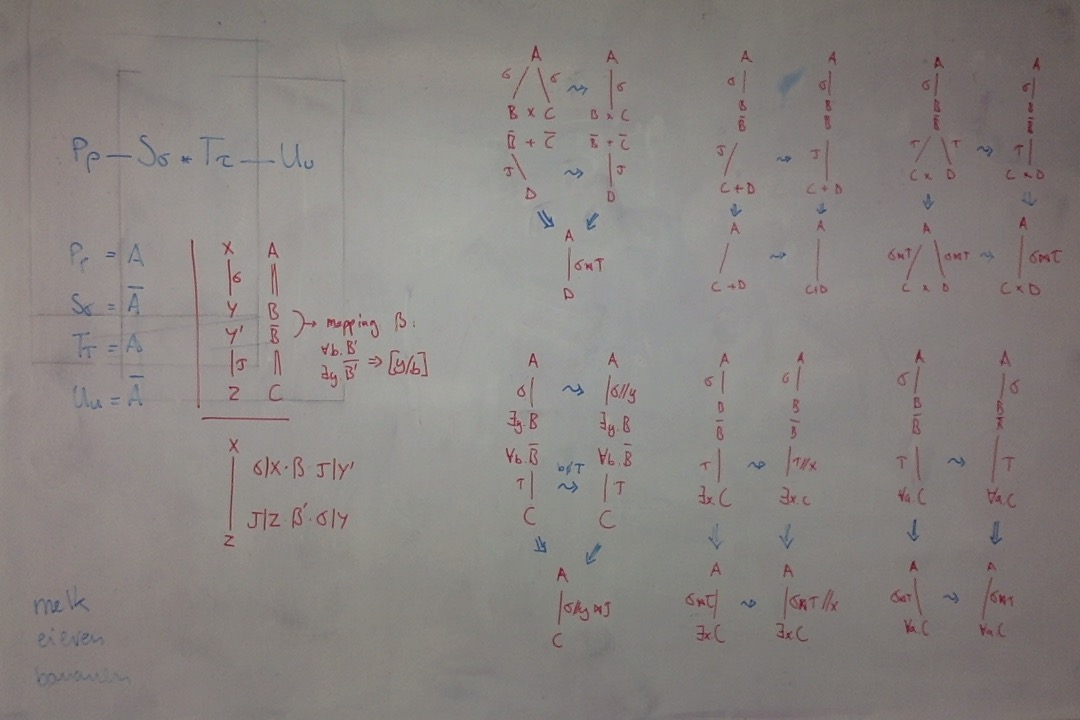
\includegraphics[scale=0.4]{normalization.jpg}


\section{Unification nets}



We define the following further operations on witness maps.
\[
\begin{tabular}{@{}lp{.75\textwidth}@{}}
	$\sigma\gen\tau$
&
	A witness map is \defn{more general} than another, 
	$\sigma\gen\tau$, if there is a map $\rho$ such that 
	$\sigma\rho=\tau$.
\\[5pt]	
	$\sigma\coh\tau$
&
	Two witness maps are \defn{coherent}, $\sigma\coh\tau$,
	if there is a map $\rho$ such that $\sigma\rho=\tau\rho$.
\\[5pt]
	$\sigma\join\tau$
&
	The \defn{join} of two witness maps $\sigma\join\tau$ is defined
	if they are coherent, and is the least map $\rho$ such that
	$\sigma\gen\rho$ and $\tau\gen\rho$.
\end{tabular}%
\]

A clean link $(P,Q)$ on two atomic formulas $P$ and $Q$ is an \defn{axiom} link if there exists a witness map $\sigma$ such that $P\sigma=\dual Q\sigma$. A clean \defn{axiom} linking is one consisting only of axiom links. 

The \defn{clean} de-sequentialization $\floor\pi$ of a proof $\pi$ is the pre-net $\net\lambda AB$ where the de-sequentialization $[\pi]=\net{\lambda_\Sigma}AB$. Observe that $\lambda$ is then an axiom linking.

To an axiom link $(P,Q)$ we assign an \defn{initial witness map} $\sigma=\init PQ$ as the least witness map in $(\gen)$ such that $P\sigma=\dual Q\sigma$. In other words, $\init PQ$ is the most general unifier ($\textsc{mgu}$) of $P$ and $\dual Q$. An axiom linking $\lambda$ with the initial witness map assigned to each link will be written $\lambda_\star$:
\[
	\lambda_\star = \{~\link PQ~\mid~(P,Q)\in\lambda~,~\sigma=\init PQ~\}~.
\]
For a pre-net $\net{\lambda_\star}AB$ we assume the \defn{exact coverage} convention, that the domain of each $\sigma(P,Q)$ is $\ex AP\cup\ex BQ$. This means a variable $x\in\varE$ in $P$ or $Q$ will be assigned at least a fresh variable name $y$.

%Together with the convention that existential variables in the range of $\sigma(P,Q)$ are fresh, 

For two witness labellings $\Sigma$ and $\Xi$ on the same linking $\lambda$, one is \defn{more general} than the other, $\Sigma\gen\Xi$, if $\Sigma(C,D)\gen\Xi(C,D)$ for every link $(C,D)\in\lambda$. We extend this to the linkings themselves: $\lambda_\Sigma\gen\lambda_\Xi$. Observe that for an axiom linking $\lambda$, the initial linking $\lambda_\star$ is the most general among the witness linkings $\lambda_\Sigma$ for any $\Sigma$.

We write $\Sigma\tau$ for the composition of every map in $\Sigma$ with $\tau$:	$\Sigma\tau(C,D) = \Sigma(C,D)\tau$. Because of the exact coverage convention, we have that, if $\lambda_\star=\lambda_\Sigma\gen\lambda_\Xi$, then $\Xi=\Sigma\tau$ for some $\tau$.



\begin{definition}
\defn{Unifying coalescence} ($\ucoal$) is the rewrite relation generated by the rules:
\[
	(\urr+i)~,~(\urr?)~,~(\urr!)
	\quad
	\text{are respectively as}
	\quad
	(\srr+i)~,~(\srr?)~,~(\srr!)
\]
except that ($\urr?$) does not require that $\sigma(x)$ is defined, plus the rule
\begin{equation}
	\net{\{\link AB^\pi,\link[\tau]AC^\phi\}}A{B\*C}
 ~\ucoal~ 
	\net{\{\link[\sigma\join\tau]A{B\*C}^\psi\}}A{B\*C}
\tag{$\urr*$}
\end{equation}

\hfill $\text{if}\quad\sigma\coh\tau~,
		\quad
		\text{where}\quad \sigma\join\tau=\sigma\rho=\tau\rho
		\quad
		\text{and}\quad \psi=~
  \vc{
   \infer  {\seq{A\sigma\rho}{B\sigma\rho\,\*\,C\sigma\rho}}  {
    \left( \vc{\deduce  [\rule{0pt}{2pt}]  {\seq{A\sigma}{B\sigma}}  \pi} \right)\rho
    &
    \left( \vc{\deduce  [\rule{0pt}{2pt}]  {\seq{A\tau}{C\tau}}  \phi} \right)\rho   
  }}~.
$ \hspace*{20pt}

\medskip

\noindent
A pre-net $\net\lambda AB$ \defn{unifying-coalesces} if it reduces in $(\ucoal)$ to a single link $\net{\{\link[\varnothing]AB\}}AB$.
\end{definition}


%A pre-net $\net\lambda AB$ \defn{strict-} or \defn{unifying-coalesces} if it reduces in $(\scoal)$ respectively $(\ucoal)$ to a single link $\net{\link[\varnothing]AB}AB$. Here, we ignore the labelling with proofs, which means in particular that we need not instate a labelling to initiate coalescence.


%A pre-net $\net\lambda AB$ \defn{coalesces}, in either relation , if it coalesces to a single clean link $\net{(A,B)^\pi}AB$. In that case, it \defn{sequentializes} It \defn{strongly coalesces} if every coalescence sequence can be extended to reach $\net{(A,B)}AB$.



\begin{definition}
An \all1 \defn{unification proof net} or \defn{unification net} is a pre-net $\net\lambda AB$ with clean axiom linking $\lambda$ such that its initial witness assignment $\net{\lambda_\star}AB$ unifying-coalesces. It \defn{sequentializes} to $\pi$ if the initial labelling $\net{\lambda^\star_\star}AB$ reduces in $(\ucoal)$ to $\net{\{\link[\varnothing]AB^\pi\}}AB$.
\end{definition}



\begin{figure}
\hrule
\par\bigskip
\[
\begin{array}{ccc}
    \vc{\begin{tikzpicture}[net]
    	\formula[y=2]{P}
    	\formula[y=1]{Q}
    	\Vlink[blue]{1,1}
    \end{tikzpicture}}
&\rightsquigarrow&    
    \vc{\begin{tikzpicture}[net]
    	\formula[y=2]{P}
    	\formula[y=1]{Q}
    	\Vlink[red,label={$~\scriptstyle{\sigma(P,\dual Q)}$}]{1,1}
    \end{tikzpicture}}
\\ \\
    \vc{\begin{tikzpicture}[net]
    	\formula[y=2]{A}
    	\formula[y=1]{B\+C}
    	\Vlink[red,label={$\scriptstyle\sigma~$},l]{1,1}
    \end{tikzpicture}}
&\rightsquigarrow& 
    \vc{\begin{tikzpicture}[net]
    	\formula[y=2]{A}
    	\formula[y=1]{B\+C}
    	\Vlink[red,label={~$\scriptstyle\sigma$}]{1,2}
    \end{tikzpicture}}
\\ \\   
    \vc{\begin{tikzpicture}[net]
    	\formula[y=2]{A}
    	\formula[y=1]{B\*C}
    	\Vlink[red,label={$\scriptstyle\sigma~$},l]{[-1]1,1}
    	\Vlink[red,label={~$\scriptstyle\tau$}]{[1]1,3}
    \end{tikzpicture}}
&\stackrel{\sigma\coh\tau}\rightsquigarrow&   
	\vc{\begin{tikzpicture}[net]
    	\formula[y=2]{A}
    	\formula[y=1]{B\*C}
    	\Vlink[red,label={~$\scriptstyle{\sigma\cup\tau}$}]{1,2}
    \end{tikzpicture}}
    
\\ \\
    \vc{\begin{tikzpicture}[net]
    	\formula[y=2]{A}
    	\formula[y=1]{\exists x.B}
    	\Vlink[red,label={~$\scriptstyle\sigma$}]{1,4}
    \end{tikzpicture}}
&\rightsquigarrow&
    \vc{\begin{tikzpicture}[net]
    	\formula[y=2]{A}
    	\formula[y=1]{\exists x.B}
    	\Vlink[red,label={~$\scriptstyle{\sigma\minus x}$}]{1,1}
    \end{tikzpicture}}
\\ \\
    \vc{\begin{tikzpicture}[net]
    	\formula[y=2]{A}
    	\formula[y=1]{\forall a.B}
    	\Vlink[red,label={~$\scriptstyle\sigma$}]{1,4}
    \end{tikzpicture}}
&\stackrel{a\,\notin\,\fv(A\sigma)}\rightsquigarrow&
    \vc{\begin{tikzpicture}[net]
    	\formula[y=2]{A}
    	\formula[y=1]{\forall a.B}
    	\Vlink[red,label={~$\scriptstyle\sigma$}]{1,1}
    \end{tikzpicture}}
\end{array}
\]
\caption{Coalescence rules}
\label{fig:coalescence}
\end{figure}


\end{document}

